%!TEX root = egalitarianism.tex

\section{Defining egalitarianism}\label{sec:definition}

We now propose the first definition of an economic measure of
\emph{egalitarianism} in cryptocurrencies. Before we present our definition, let
us first state the desiderata of such a definition. First of all, we would like
a definition which allows concrete measurements to be performed on
cryptocurrencies and data to be extracted in a manner that is quantitative and
not vague. The claims for egalitarianism in various cryptocurrencies have been,
thus far, hand wavy and comparisons have used rhetoric which does not include
exact data. As such, different cryptocurrencies have claimed that each is more
egalitarian than the other, but these claims have not been demonstrated or have
remained inconclusive. Intuitively, a definition of egalitarianism wishes to
measure how much the amount of money generated through block generation by the
investment of a \emph{poor dollar} differs from that generated by the investment
of a \emph{rich dollar}. We thus desire a measure which, for a particular
cryptocurrency, extracts a value between $0$ and $1$, where $0$ indicates a
complete \emph{lack of egalitarianism} and that a rich dollar is infinitely more
powerful than a poor dollar, while $1$ indicates \emph{perfect egalitarianism}
in which a rich dollar and a poor dollar have exactly equal power in terms of
cryptocurrency generation.

As a means towards our egalitarianism definition, we first define the
\emph{egalitarian curve} $f$ of a cryptocurrency. The curve is plotted with a
fixed investment duration in mind. In this paper, we use a duration of 1 year.
Of course, curves of different cryptocurrencies can be compared only if they
use the same duration. The curve plots the available financial capital available
for investment on the horizontal axis, denominated in USD (given that we explore
a small investment duration, it makes little difference whether these are
nominal or real, as long as they are the same when applying comparisons). The
vertical axis plots the Return On Investment (ROI), which measures the
cryptocurrency amount that can be freshly generated in the investment duration,
given an optimal allocation of the financial capital. Note that we require that
the Return On Investment is necessarily \emph{freshly generated} cryptocurrency;
thus, it must be newly mined or minted. Of course, purchasing cryptocurrency
which has already been generated is an investment option, but it is immaterial
to our egalitarianism definition, which focuses on measuring the egalitarianism
of freshy generated cryptocurrency.

\begin{definition}[Egalitarian curve]
  Given a cryptocurrency $c$, an investment period duration $d$, a minimum
  capital $v_0$ and a maximum capital $v_1$, we define the
  \emph{egalitarian curve}
  $f_{c,d,v_0,v_1}: [v_0, v_1] \longrightarrow \mathbb{R}^+$ of $c$ for
  duration $d$ covering the range of capital $v_0 \cdots v_1$ is defined as:

  \[
  f_{c,d,v_0,v_1}(v) = \frac{\max_B{\mathbb{E}[B(v)]} - v}{v}
  \]

  Where the maximum is taken across all investment strategies $B$ which return
  the freshly generated coins which remain unspent for a given initial capital
  $v$ (and, hence, denotes the optimal strategy). The expectation is taken with
  the blockchain execution as a random variable, as returns vary by execution.
\end{definition}

We remark that we do allow strategies to reinvest capital. As an example,
returns earned from mining rewards can be reinvested in electricity costs for
future mining. Furthermore, for unit consistency, we assume the strategy $B(v)$
returns the freshly generated coins in the same units as the capital $v$ was
given in, such that $f$ represents a ROI.

It is now easy to define the \emph{ideal egalitarian curve}. In this curve, the
ROI remains the same regardless of capital invested. Under these ideal
conditions, the amount of freshly generated cryptocurrency will be exactly
proportional to the money invested. Thus, the ideal curve is any constant curve,
as depicted in Figure~\ref{fig:ideal}. It may at first be hoped that the
egalitarian curve of an ideal cryptocurrency could even be decreasing, meaning
that the poor are able to generate more currency for every dollar they invest.
However, one can quickly see that, in decentralized cryptocurrencies, it is
impossible to hope for something better than the constant curve. The reason is
that decentralized cryptocurrencies allow anonymous generation of new
identities. Thus, if the curve were ever to have a negative slope, a rich
investor could split their investment into smaller ones and invest each of them
individually to achieve a higher gain. By the definition of the curve, which
mandates that it depicts the ROI of an \emph{optimal} investment, this would be
a contradiction.

\begin{figure}[H]
    \caption{The ideal egalitarian curve of an ideal cryptocurrency.}
    \centering
    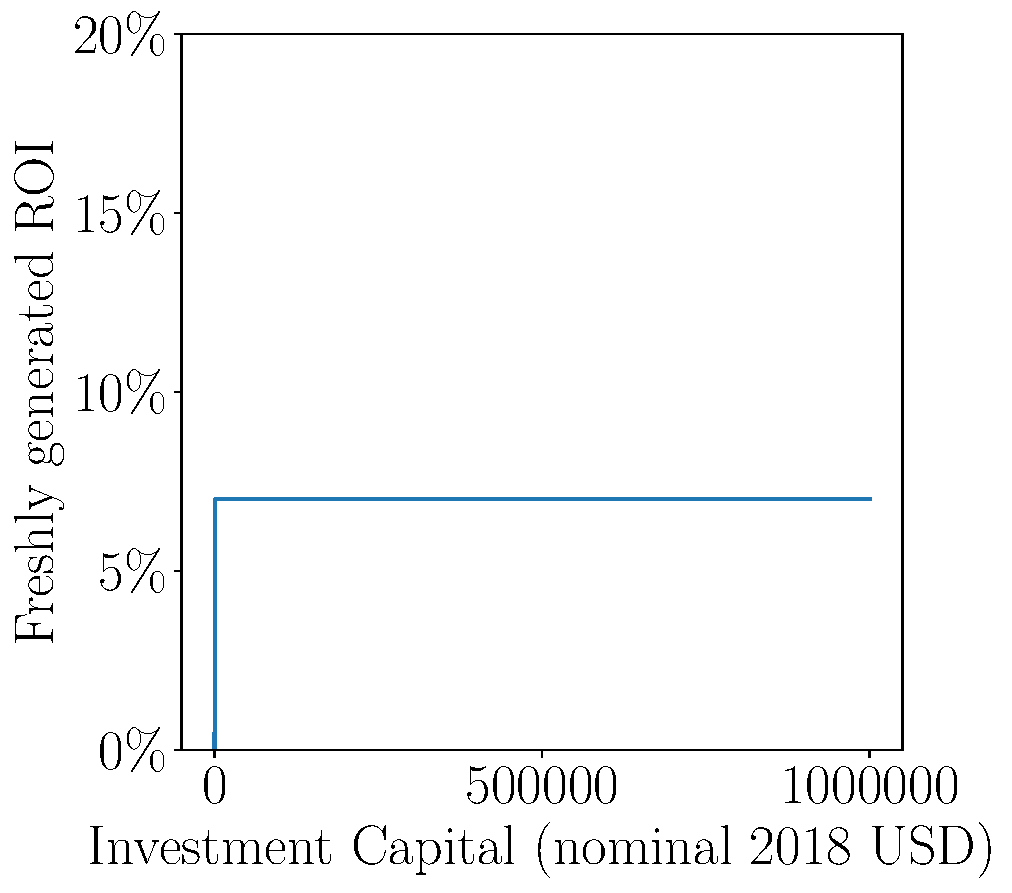
\includegraphics[width=0.75 \columnwidth,keepaspectratio]{figures/ideal.pdf}
    \label{fig:ideal}
\end{figure}

Now that we have defined the egalitarian curve, we can define egalitarianism
as a concrete number. We begin by considering the initial capital $v$ as a
random variable following a certain distribution $\mathcal{D}$. Egalitarianism
is defined as the variance of the expected ROI when the capital is chosen from
the given distribution.

\begin{definition}[Egalitarianism]
  Given a cryptocurrency $c$, an investment period duration $d$ and an initial
  capital distribution $\mathcal{D}$, we define the \emph{egalitarianism} $e$ of $c$
  for investment duration $d$ under initial capital distribution $\mathcal{D}$
  as follows:

  \[
    e_{c,d,\mathcal{D}} = -\textsf{Var}_{v \gets \mathcal{D}}[f(v)]
  \]

  where $f$ is the egalitarian curve of $c$ for duration $d$ and the support of
  $\mathcal{D}$ is $[v_0, v_1]$.
\end{definition}

The intuition behind this definition is that, to have egalitarianism, the ROI
must remain the same across different capital investments. As such, any
deviation from the mean is non-egalitarian. Our notion allows the comparison of
the egalitarianism of different cryptocurrencies. Naturally, if the
egalitarianism of a certain cryptocurrency is \emph{higher} than another's, we
say that the former is \emph{more egalitarian} than the latter. Of course, to be
accurate, such comparisons must only be made after fixing the parameters $c$
and $d$ as well as the initial capital distribution $\mathcal{D}$.
